\section{Evaluation Environment}
\label{sec:testingEnv}

%% 
%% Leave first page empty
\thispagestyle{empty}

Our evaluation environment runs tests on WebRTC. Figure~\ref{fig:evaluation_arch} describes the functional blocks used for a simple video call over WebRTC.

 \begin{figure}[h]
  \centering
    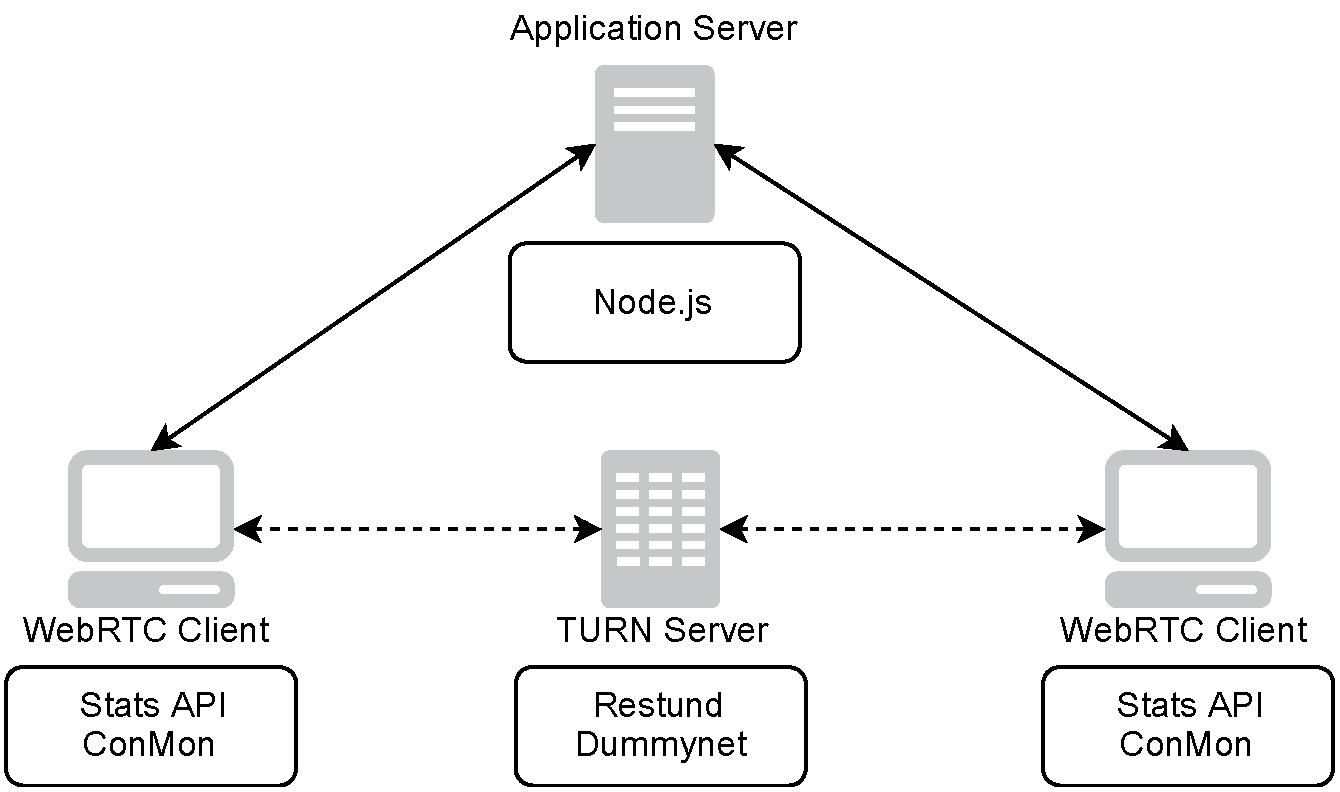
\includegraphics[width=1\textwidth]{./figures/evaluation_arch.pdf}
      \caption[Description of simple testing environment topology for WebRTC]{Description of simple testing environment topology for WebRTC.}
	\label{fig:evaluation_arch}
\end{figure}

\subsection{WebRTC client}

WebRTC clients are virtual machines that run a lightweight version of Ubuntu (Lubuntu\footnote{https://wiki.ubuntu.com/Lubuntu}) with 2GB of RAM and one CPU. This light version removes graphic acceleration providing better results in performance than compared with other distributions due to the virtualization of the graphic card. 

Clients run Chrome Dev version 27.01453.12 as a WebRTC capable browser. To avoid unexpected results due to a bug in the {\it Pulse Audio} module of Ubuntu that controls audio input in WebRTC\footnote{https://bugs.launchpad.net/ubuntu/+source/pulseaudio/+bug/1170313}, calls are done with video only, the amount of audio transferred due to the echo cancelation systems can be neglected.

\subsubsection{Connection Monitor}

Connection Monitor [{\it ConMon}] is a command line utility that relies on the transport layer and uses {\it libpcap}\footnote{http://www.tcpdump.org/} to sniff all the packets that to go a certain interface and port~\cite{singhConMon}. This utility is designed specifically to detect and capture RTP/UDP packets. {\it ConMon} detects and saves the header but discards the payload of the packet keeping the information we need for calculating our performance indicators.

Typically we run the {\it PeerConnection} between two devices and start capturing those packets using {\it ConMon} at each endpoint. The {\it PeerConnection} carries real media so the environment for testing is going to be a precise approach to a real scenario of WebRTC usage.

{\it ConMon} captures are be saved into different files allowing us to plot separate different stream rates and calculate other parameters such as delay with post processing. {\it ConMon} allows us to compare network layer and JavaScript API monitoring tools, as {\it ConMon} is working directly over the network interface and avoids all the processing that the browser internals do to send the stats to the JavaScript statistical API. Figure~\ref{fig:onetooneWifiRTCConMon} represents one video stream from the same call as Figure~\ref{fig:onetooneWifiRTC} captured from the {\it ConMon} application.

 \begin{figure}[h]
  \centering
    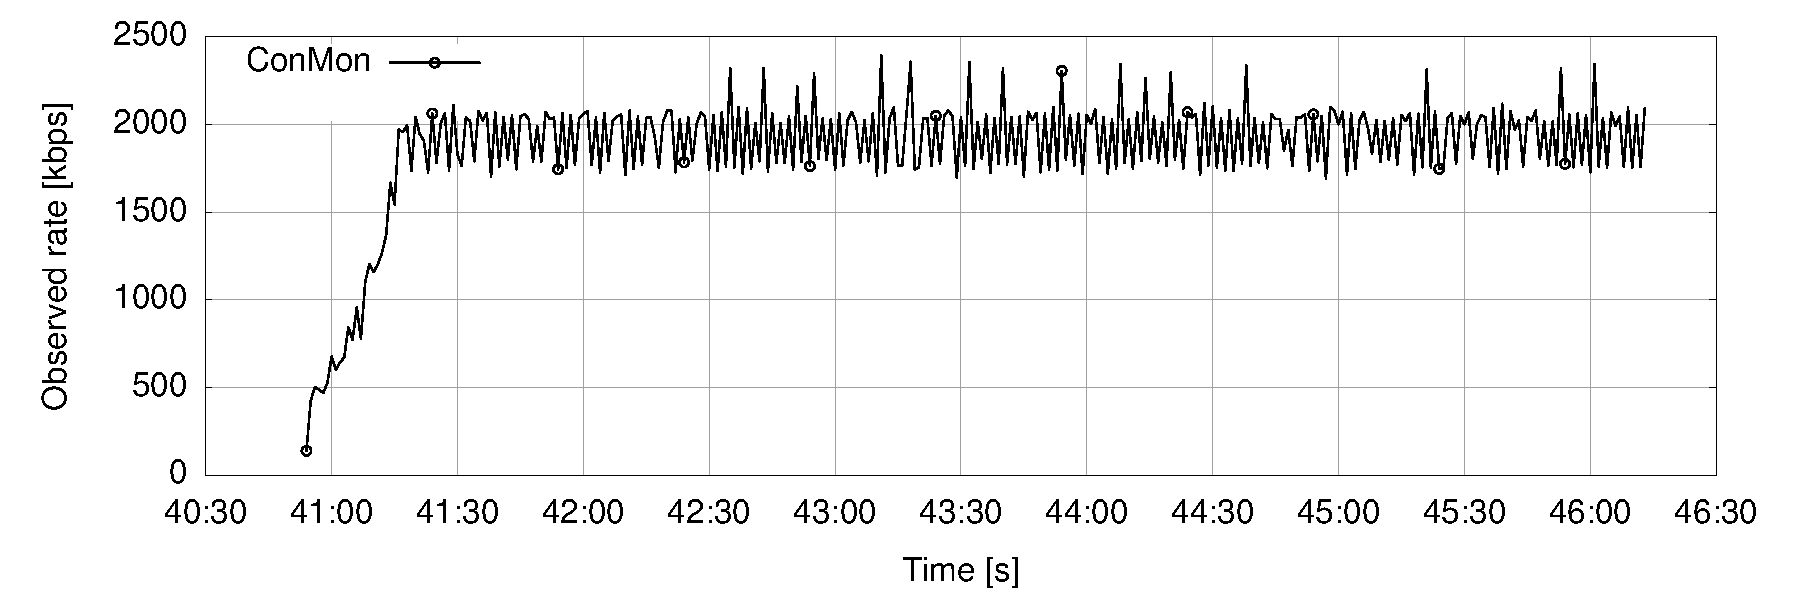
\includegraphics[width=1\textwidth]{./figures/onetooneWiFiConMon.pdf}
      \caption[Point-to-point WebRTC video stream throughput graph using ConMon over public WiFi at the network layer]{Point-to-point WebRTC video stream throughput graph using ConMon over public WiFi at the network layer.}
	\label{fig:onetooneWifiRTCConMon}
\end{figure}

The capture from {\it ConMon} is very accurate as it analyzes all the packets that go through an interface, this data is processed and averaged for a each period of one second. 

%This process might output some fluctuations on the graph that could distort the reality in some cases..

Furthermore, {\it ConMon} is used to provide OWD and RTT calculations for our tests, in order to do this we assure a proper synchronization between local clocks in all the peers. This is done by using the sequence number of all RTP packets captured and subtracting the timestamp stored from both sides, no RTCP data is used in this analysis.

\subsubsection{Stats API}

WebRTC statistical API provides methods to help developers access the lower layer network information at the receiver, those methods return all different types of statistics and performance indicators that we use to build high level JavaScript {\it Stats API}. When using those statistics we process all the output data to obtain the metrics for WebRTC.

This system works in parallel with {\it ConMon}, both of them can provide similar results of some metrics and the comparison might be interesting to check the differences between the browser API and an interface layer capture. By communing both methods we can verify the results and accuracy of the metrics.

The method used for {\it Stats API} is the {\it RTCStatsCallback} that returns a JSON object that has to be parsed and manipulated to get the correct indicators, this object returns as many arrays as streams available in a {\it PeerConnection}, two audio and video~\cite{editorWebRTCdraft} objects per {\it PeerConnection} when having a point-to-point call. This data is provided by the lower layers of the network channel extracting the information from the RTCP packets that come multiplexed in the same network port~\cite{rtpusageIETF}.

{\it RTCStatsCallback} is the mechanism of WebRTC that allows the developer to access different metrics, as this is still in an ongoing discussion, the stats report object has not been totally defined and can slightly change in the following versions of the WebRTC API, methods involved in the {\it RTCStatsCallback} are available on the W3C editors draft~\cite{editorWebRTCdraft}. 

We have built a high level {\it Stats API} that use those statistics from the {\it RTCStatsCallback} to calculate the RTT, throughput, loss rate and encoding/decoding rate for the different streams that are being processed. Those stats are saved into a file or sent as a JSON object to a centralized monitoring system. Our JavaScript API grabs any {\it PeerConnection} passed through the variable and starts looping a periodical iteration to collect those stats and, either plot them or save them into an array for post-processing. 

Figure~\ref{fig:onetooneWifiRTC} represents an example of a captured call between two browsers in two different machines, Mac and Ubuntu, the call was made over Wifi network with no firewall but with unknown cross traffic on it. The measures were directly obtained from the {\it Stats API} we built and post-processed using {\it gnuplot}\footnote{http://www.gnuplot.info/}.

 \begin{figure}[h]
  \centering
    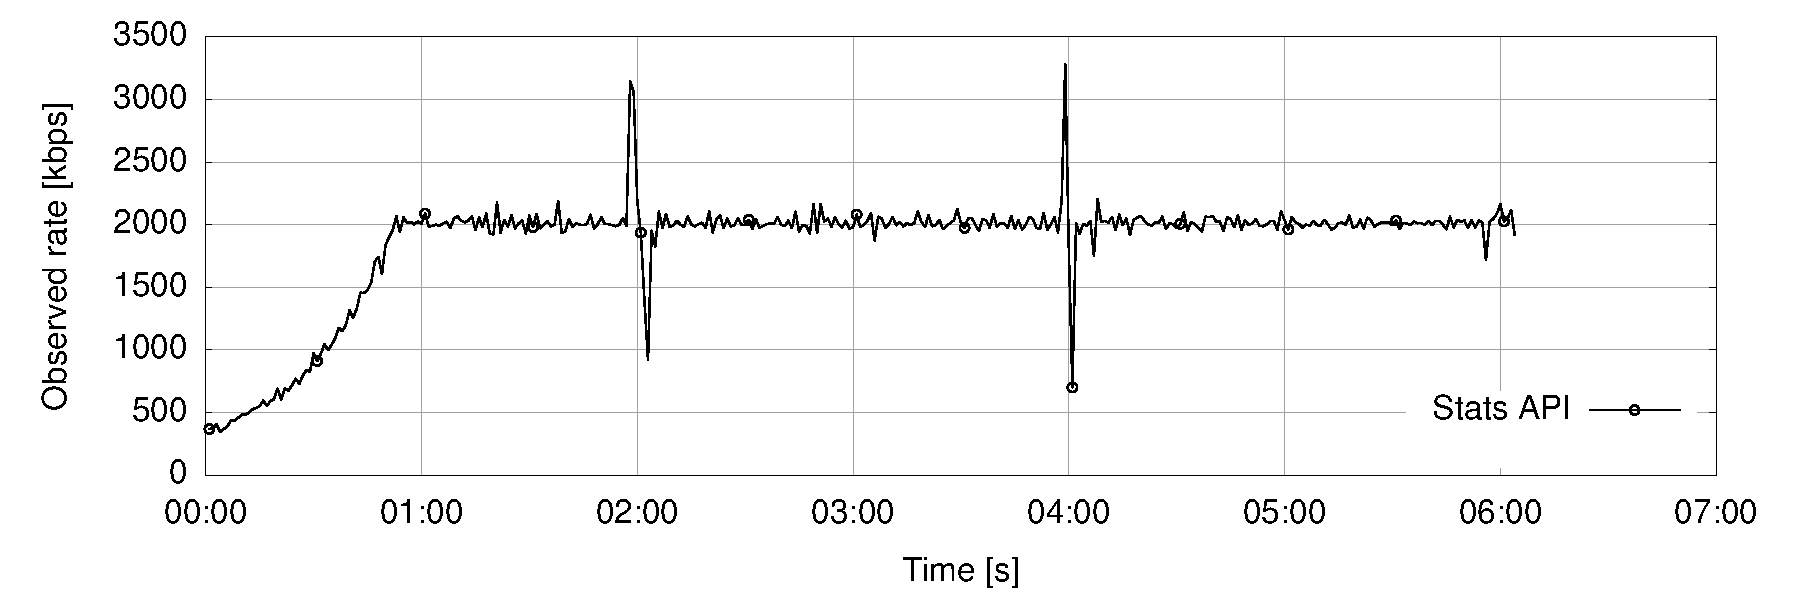
\includegraphics[width=1\textwidth]{./figures/onetooneWifiStatsRTC.pdf}
      \caption[Point-to-point WebRTC video call total throughput graph using {\it Stats API} over public WiFi]{Point-to-point WebRTC video call total throughput graph using {\it Stats API} over public WiFi.}
	\label{fig:onetooneWifiRTC}
\end{figure}

Figure~\ref{fig:onetooneWifiRTC} plots the overall bandwidth of the call, this means that the input/output video and audio are measured together to check how much total bandwidth is being consumed over the duration of the call, as it is using RTCP packets to deliver the metrics to the {\it Stats API}, it takes a while to reach the average rate value until congestion mechanisms adapt the used rate to the network conditions. We can then plot all the different streams together to get an idea of how much bandwidth the {\it PeerConnection} is consuming.

% \begin{figure}[h]
%  \centering
%    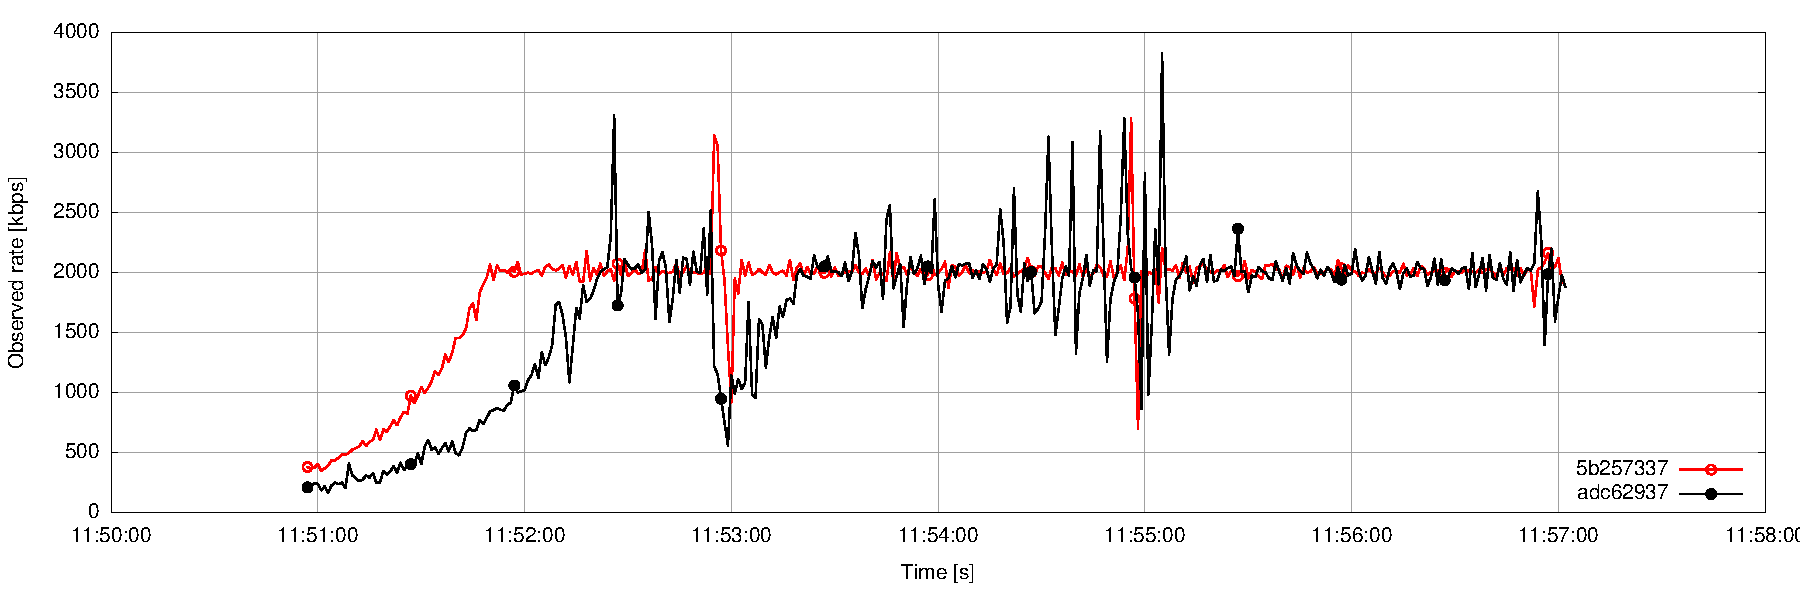
\includegraphics[width=1\textwidth]{./figures/onetooneWiFIStatsVideoStreams.pdf}
%      \caption[Point-to-point WebRTC input/output video throughput graph using Stats API over public WiFi]{Point-to-point WebRTC input/output video throughput graph using Stats API over public WiFi.}
%	\label{fig:onetooneWifiRTCVideoStreams}
%\end{figure}
%
%Figure~\ref{fig:onetooneWifiRTCVideoStreams} shows the two video streams captured from the same machine, one is outgoing the local video stream meanwhile the second stream is the incoming video stream from the other peer. We have built a flexible processing system that allows us to capture and analyze all the possible combinations of streams and metrics. The timing used for the capture is provided by the TimeStamp available on the RTCP. The average bandwidth used in this scenario of point-to-point call in a standard wireless network is around 2000 Kbps per video stream. Both figures are plotted from the same original call.

% \begin{figure}[h]
%  \centering
%    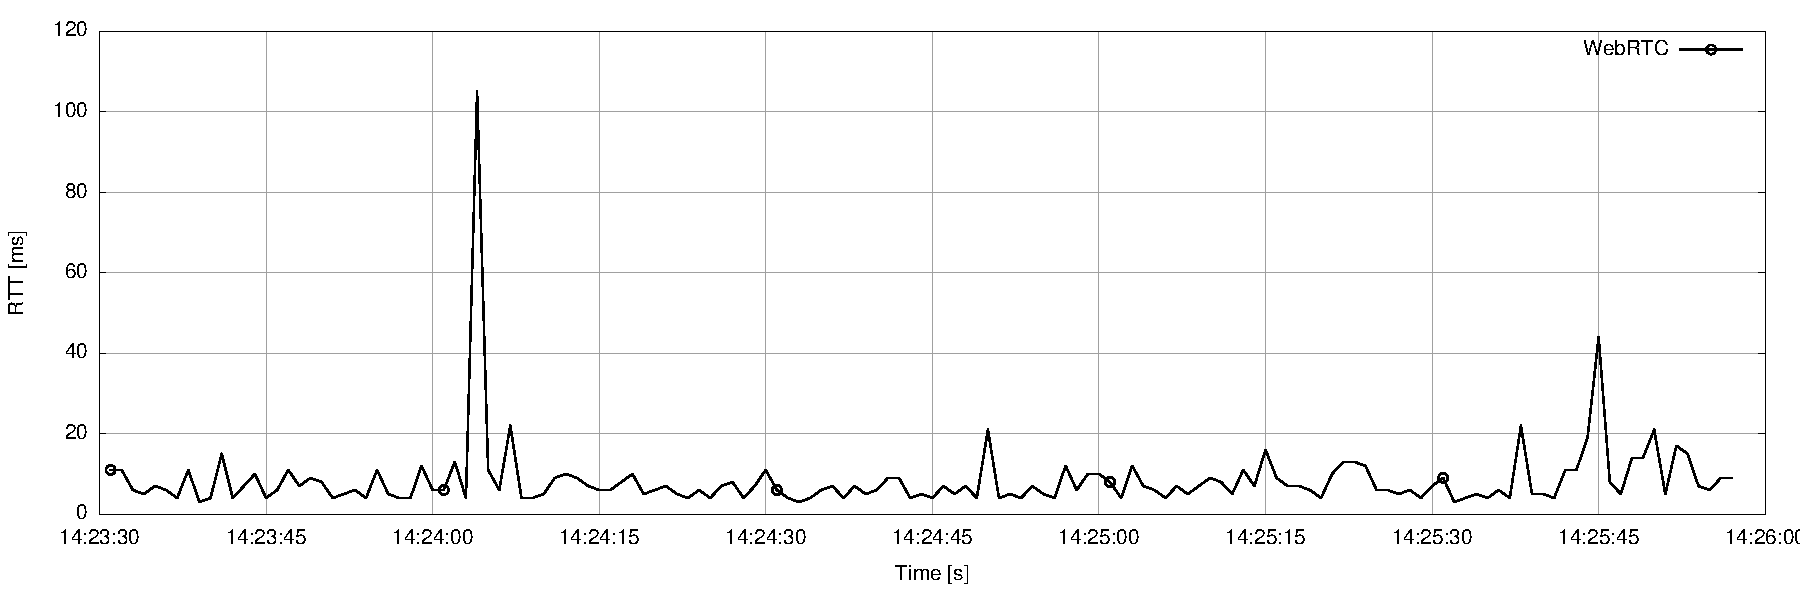
\includegraphics[width=1\textwidth]{./figures/p2prttexample.pdf}
%      \caption[Point-to-point WebRTC RTT measure using Stats API over public WiFi]{Point-to-point WebRTC RTT measure using Stats API over public WiFi.}
%	\label{fig:p2prttexample}
%\end{figure}

%Our Stats API also provides extra information such as RTT and loss rate, RTT should be provided natively by the WebRTC %method but it is possible to calculate it by using the DataChannel provided by the PeerConnection, we are using this %channel to send a UNIX TimeStamp object to the other peer and take it back, when the round trip is finished we compare it %with the actual millisecond and obtain the total RTT.

%Figure~\ref{fig:p2prttexample} represents the capture of a video call between two peers, if we are able to process the JavaScript forwarding function in an optimal way this would led to a precise RTT measurement hack without the need of Stats method.

\subsubsection{Analysis of tools}

{\it Stats API} and {\it ConMon} measure the same metrics but from different layers of the operating system, this provides us some extra information in order to see how the our high level {\it Stats API} works and if it is reliable and accurate.

However, due to the periodical capture method, the output can produce strange plots as the information regarding to the next data period could be stored in the previous one when processing the averaged data on the system. This is an accuracy problem that cannot be easily solved, when looking at the graph, it is important to observe if two peaks (positive and negative) get compensated by each other, this would mean that the data has not been allocated to the correct period when plotted. This accuracy error is a problem that can be observed when comparing both {\it ConMon} and {\it Stats API} capture in Figure~\ref{fig:delay_mesh_peer1}. 

A second problem that we could face is the time it takes to the OS to process the stats form the RTCP packet and send them to the upper browser layer, at the receiver some of the stats are based on the current measurement of the metrics not in the RTP Receiver Report. Figure~\ref{fig:p2pincommingStatsConmonWifi} and~\ref{fig:p2poutgoingStatsConmonWifi} plot two video streams being captured from Stats API and {\it ConMon}.

\begin{figure}[h]
        \centering
        \begin{subfigure}[b]{0.5\textwidth}
                \centering
                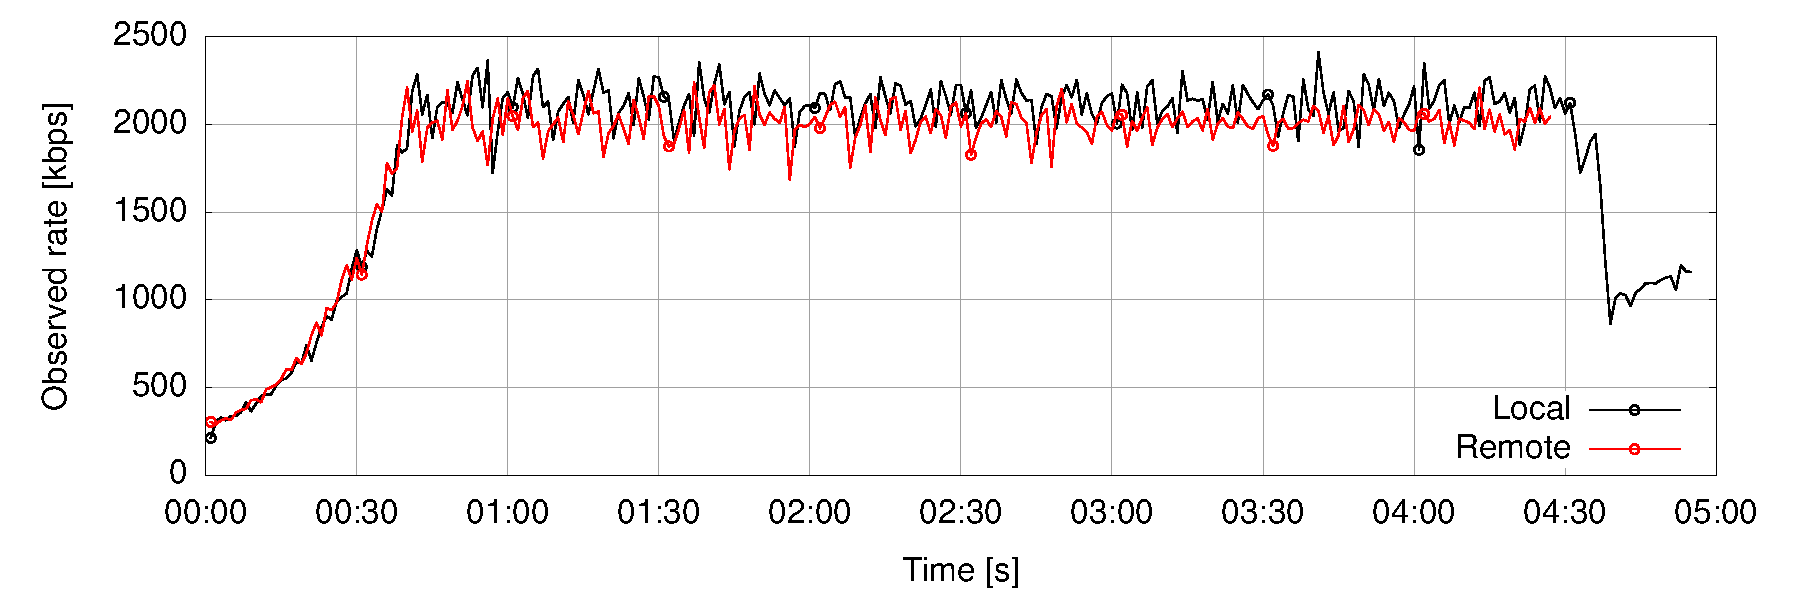
\includegraphics[width=\textwidth]{./figures/p2p_incomming_cable_sample.pdf}
               \caption[Incomming stream]{Incomming stream.}
			\label{fig:p2pincommingStatsConmonWifi}
        \end{subfigure}%
        ~ %add desired spacing between images, e. g. ~, \quad, \qquad etc.
          %(or a blank line to force the subfigure onto a new line)
        \begin{subfigure}[b]{0.5\textwidth}
                \centering
                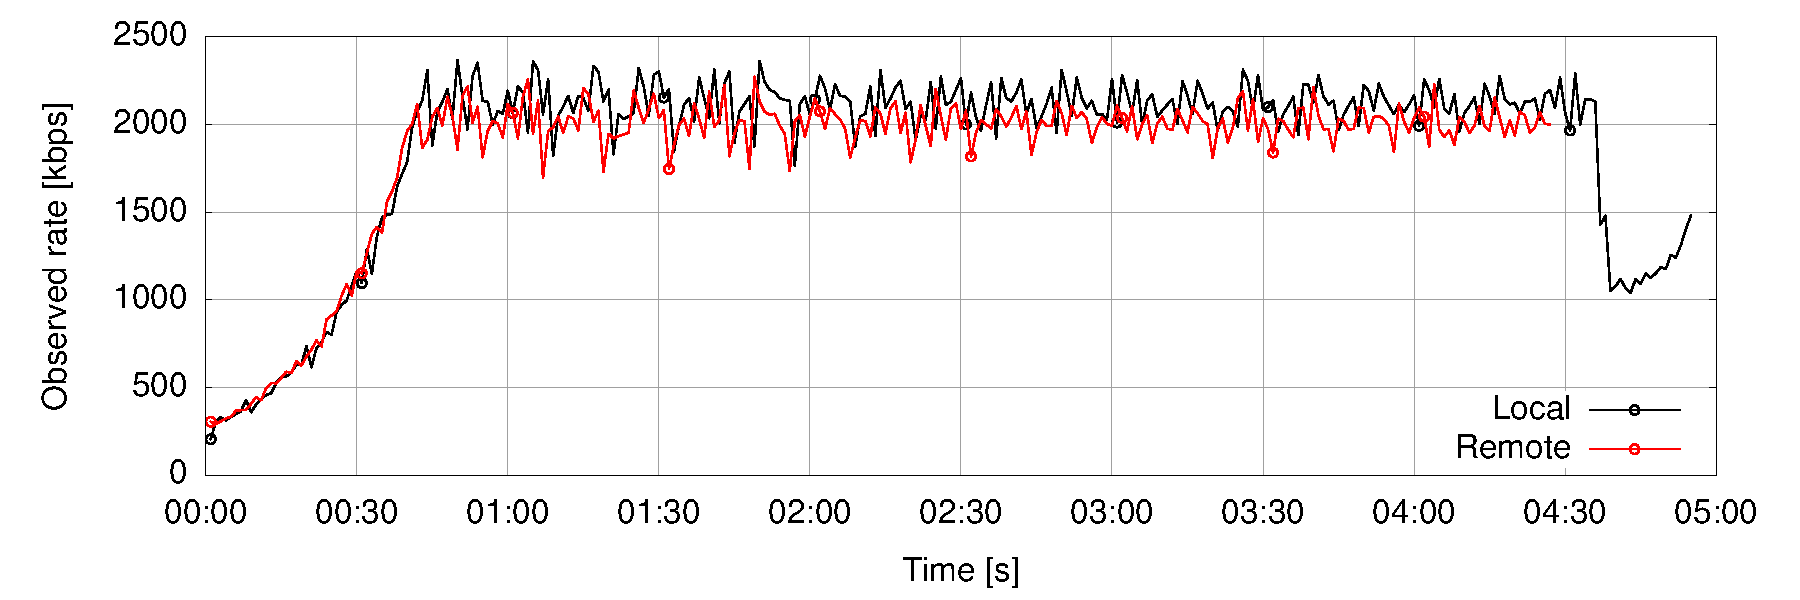
\includegraphics[width=\textwidth]{./figures/p2p_outgoing_cable_sample.pdf}
               \caption[Outgoing stream]{Outgoing stream.}
			\label{fig:p2poutgoingStatsConmonWifi}
	        \end{subfigure}
        \caption[P2P video stream comparison between {\it ConMon} and {\it Stats API}]{P2P video stream comparison between {\it ConMon} and {\it Stats API}.}
        \label{fig:p2pStatsConmon}
\end{figure}

Figure~\ref{fig:p2pStatsConmon} represents the incoming media stream from the other peer, we can see the little overhead that is not captured by the {\it Stats API} interface, as it just reads the bytes inside the payload of the packet. All the overhead is not considered when calculating the rate though {\it Stats API}. We can conclude that the real rate that WebRTC use is going to be defined by the result of {\it ConMon} instead of {\it Stats API}, but {\it Stats API} is going to be an accurate approach.

\subsection{Automated testing}

For our test scenario we have considered two options, manual and automated testing. The first test environment does not give as much accuracy due to the impossibility to iterate the test many times for the same configuration, if the second option is available the results can be averaged between all the iterations resulting in an accurate result.

In some environments, we won't be able to perform automated testing, when this happens the results won't be as accurate but they can provide a good approximation to the averaged value.

One of the main issues when building a test scenario is the media provided to the {\it GetUserMedia} input, this media must be as close to reality as possible without using a real webcam. Google Chrome provides a fake video flag that can be activated by adding {\it --use-fake-device-for-media-stream}\footnote{http://peter.sh/experiments/chromium-command-line-switches/} parameter, this video though, does not produce enough rate for our purposes.

%\begin{figure}[h]
%	\begin{minipage}{.5\textwidth}
%		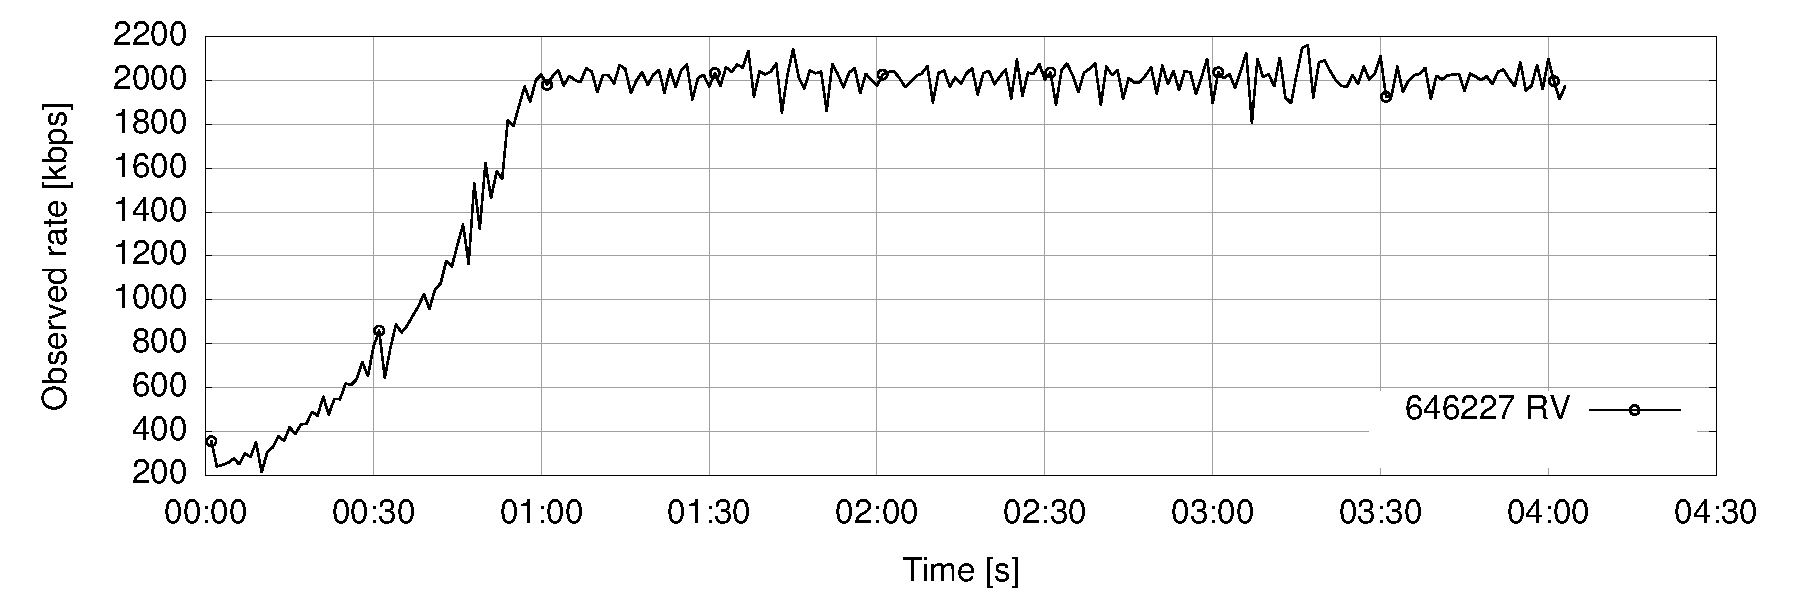
\includegraphics[width=1\textwidth]{./figures/realVideoChrome.pdf}
%			\caption[Video stream bandwidth between two peers using webcam]{Video call bandwidth between two peers using webcam.}
%			\label{fig:realVideoChrome}
%	 \end{minipage}
%	 \begin{minipage}{.5\textwidth}
%		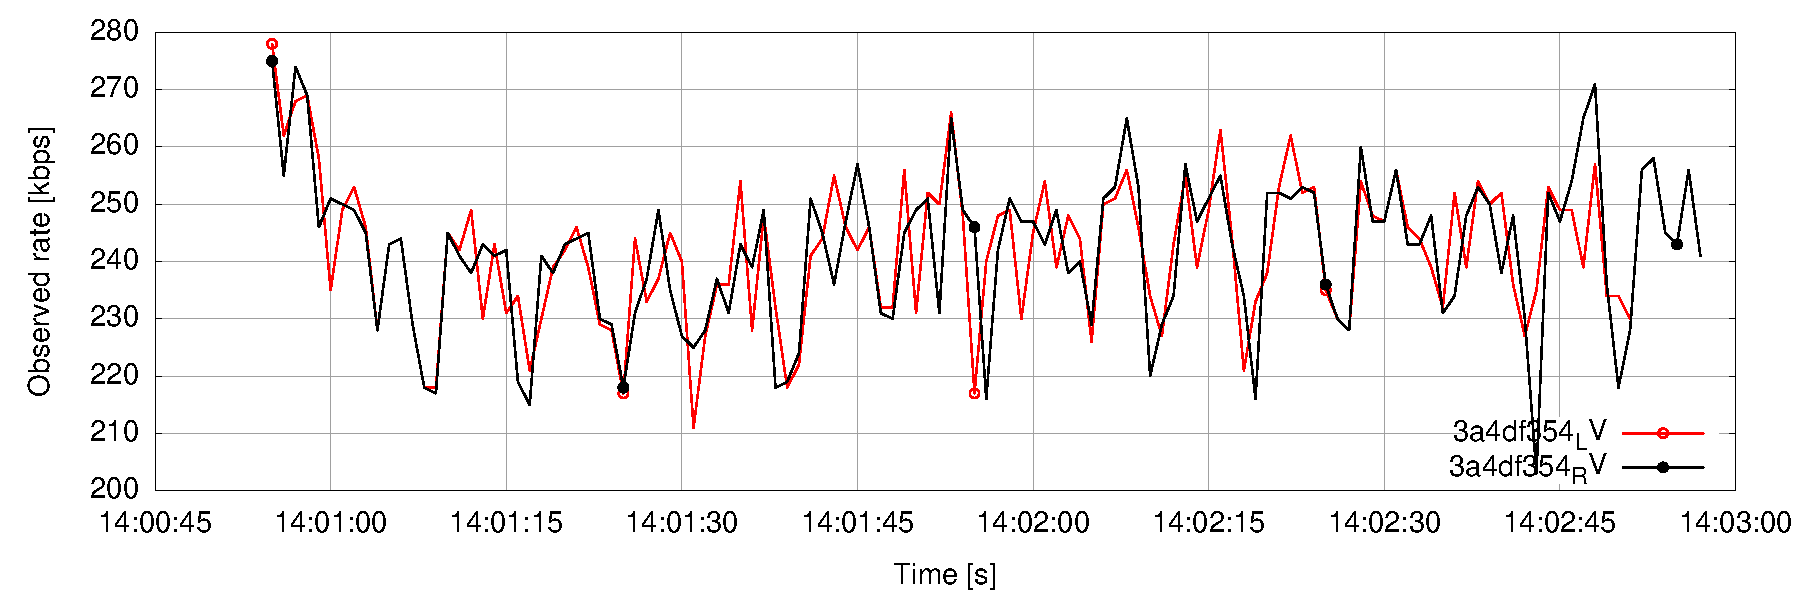
\includegraphics[width=1\textwidth]{./figures/automatedVideoChrome.pdf}
%			\caption[Video stream bandwidth between two peers using fake video]{Video stream bandwidth between two peers using fake video.}
%			\label{fig:automatedVideoChrome}
%	 \end{minipage}
%\end{figure}

 \begin{figure}[h]
  \centering
   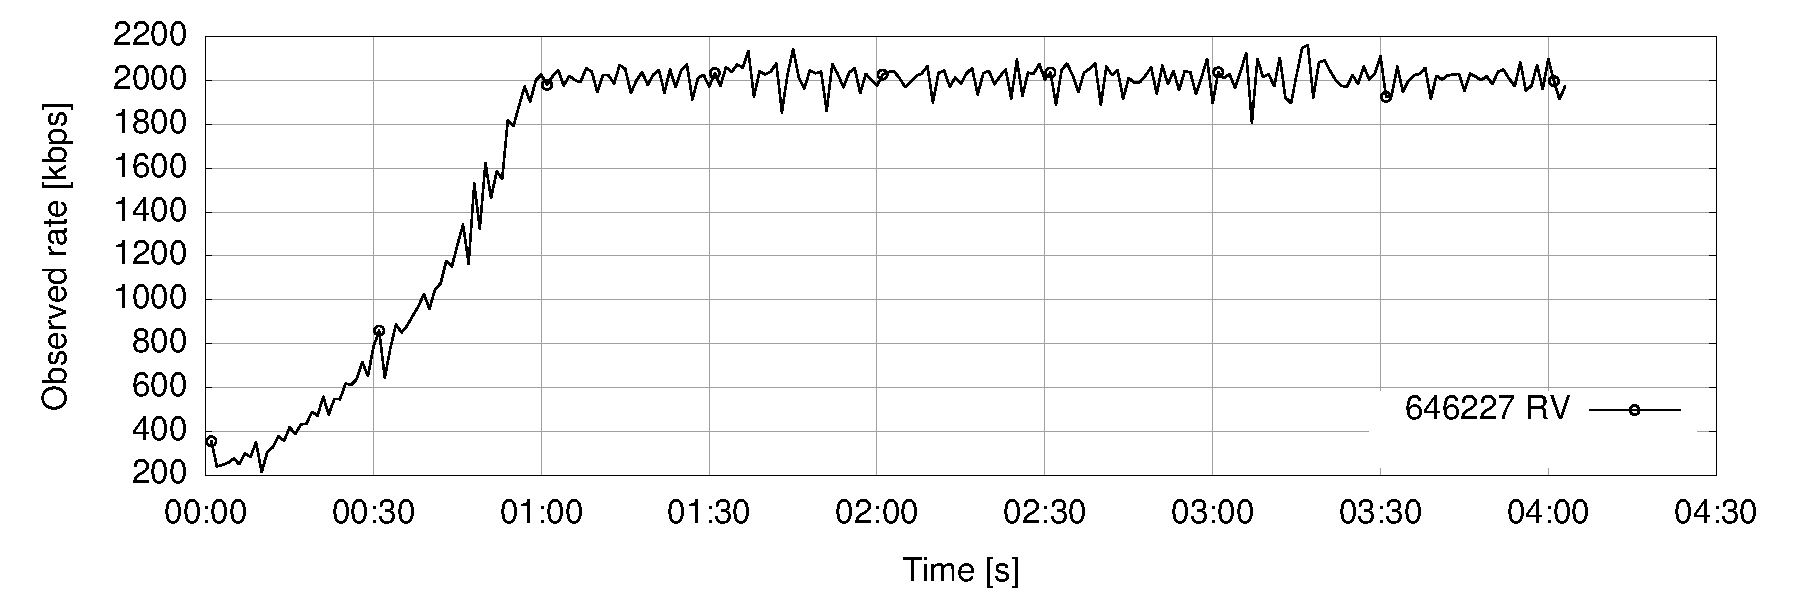
\includegraphics[width=1\textwidth]{./figures/realVideoChrome.pdf}
     \caption[Video stream rate with SSRC 0x646227 captured using {\it Stats API} and webcam input]{Video stream rate with SSRC 0x646227 captured using {\it Stats API} and webcam input.}
	\label{fig:realVideoChrome}
%\end{figure}
 %\begin{figure}[h]
  \centering
	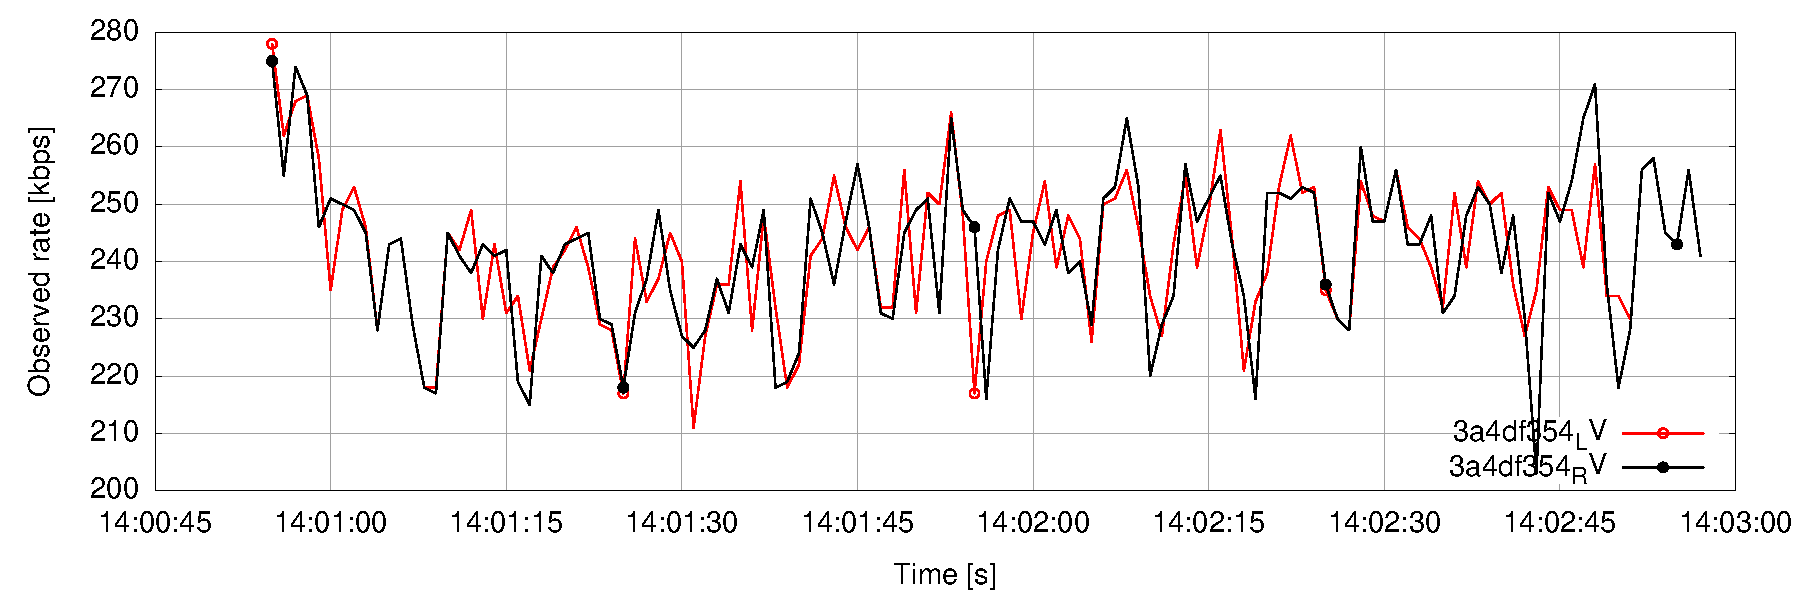
\includegraphics[width=1\textwidth]{./figures/automatedVideoChrome.pdf}
	\caption[Video stream rate with SSRC 0x3a4df354 captured using {\it Stats API} and Chrome default fake content]{Video stream rate with SSRC 0x3a4df354 captured using {\it Stats API} and Chrome default fake video input.}
	\label{fig:automatedVideoChrome}
\end{figure}

Figure~\ref{fig:realVideoChrome} represents the approximate bandwidth that a real video call uses when sending media to another peer, that capture shows the same stream captured from the origin and receiver {\it StatsAPI} perspective. The adequate rate rises to 2000 Kbps. On the other hand, Figure~\ref{fig:automatedVideoChrome} represents the scenario but using the built-in fake video in both clients, the rate for this case drops to an average of 250 Kbps. 

Both figures (\ref{fig:realVideoChrome} and~\ref{fig:automatedVideoChrome}) print one unique stream, identified with the Synchronization Source identifier (SSRC) \nomenclature{SSRC}{Synchronization Source identifier}, but from the sender and receiver perspective, {\it LV} identifies the source capture and {\it RV} the receiver stream rate. 

Comparing global output from Figures ~\ref{fig:realVideoChrome} and ~\ref{fig:automatedVideoChrome}, we can see that the obtained rate is very different concluding that we cannot use {\it --use-fake-device-for-media-stream} flag for our testing environment. The reason is that Google Chrome uses a bitmap system to draw the figures and components that will be rendered in the video tag and sent over the {\it PeerConnection}, this means that the amount of encoding and bandwidth used will be low compared to a real webcam as the media sent over with fake video is minimum.

To address this issue of the media streaming for our automated devices, we have built a fake input device on the peers, the procedure is described in Appendix~\ref{sec:fakeVideo}.

 \begin{figure}[h]
  \centering
    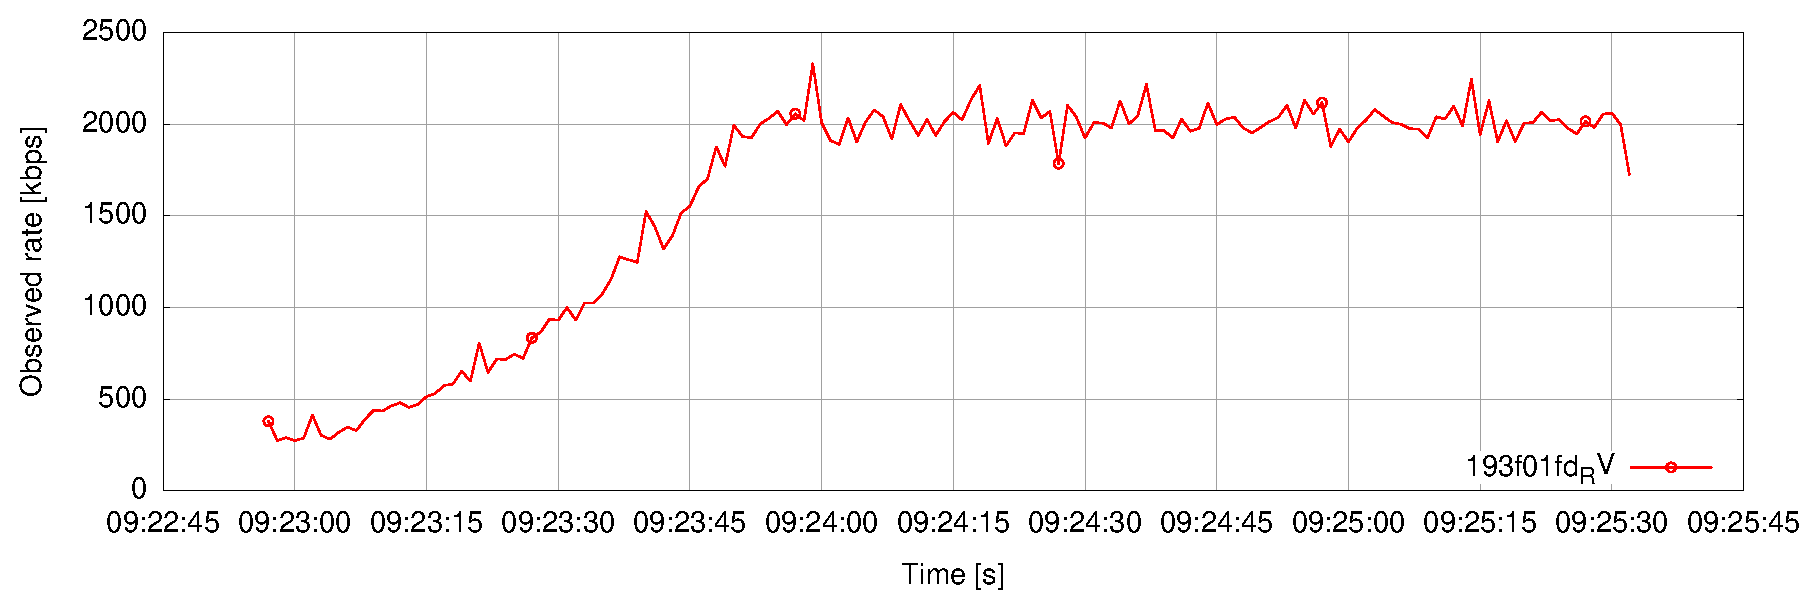
\includegraphics[width=1\textwidth]{./figures/testV4L2niklas.pdf}
      \caption[Video stream bandwidth using V4L2Loopback fake YUV file]{Video stream bandwidth using V4L2Loopback fake YUV file.}
	\label{fig:testV4L2niklas}
\end{figure}

Figure~\ref{fig:testV4L2niklas} represents the bandwidth of a fake video stream measured by our {\it Stats API} using an YUV\footnote{YUV is a color space that encodes video taking human perception into account, typically enabling transmission errors or compression artifacts to be more efficiently masked by the human perception than using RGB-representation.} video captured from a Logitech HD Pro C910 as source, resolution is 640x480 at a frame-rate of 30 fps. 

Results can be compared between Figure~\ref{fig:testV4L2niklas} and~\ref{fig:realVideoChrome}, both average rate output is approximately 2000 Kbps, which means that this procedure is a good approach to a real webcam. 

The combination of the previous fake video setup and multiple Secure Shell \nomenclature{SSH}{Secure Shell} scripts enables the automation mechanisms to run multiple tests without the need of multiple physical devices.

\subsection{TURN Server}

Our TURN server is used to pipe all the media as a relay, allowing us to apply the network constraints required for the tests to a centralized node, this machine is a Ubuntu Server 12.04 LTS with a tuned kernel adapted to perform better with {\it Dummynet}.

The TURN daemon we use is called {\it Restund}, which has been proven to be reliable for our needs, this open source STUN/TURN server works with {\it MySQL} database authentication~\cite{restund}. We have modified the source in order to have a hardcoded password making it easier for our needs.

To do so, we need to modify {\it db.c} file before compiling. Content of  method {\it restund\_get\_ha1} has to be replaced with the following line of code, where XXX is username and YYY the password we use for the TURN configuration.

\lstset{language=C}
\begin{lstlisting}[caption=Forcing a hardcoded password in our TURN server]
md5_printf(ha1, "\%s:\%s:\%s", "XXX", "myrealm", "YYY");
\end{lstlisting}

Furthermore, in order to force WebRTC to use TURN candidates we need to replace the WebRTC API server identification with our TURN machine by doing:

\lstset{language=JavaScript}
\begin{lstlisting}[caption=Configuring our TURN server in WebRTC]
var pc_config = {
	"iceServers": [{url: "turn:XXX@192.168.1.106:3478", credential:"YYY"}]
};
\end{lstlisting}

The previous object is provided to the {\it PeerConnection} object enabling the use of TURN.

The IP address points to our TURN server and the desired port (3478 by default), now all candidates are obtained through our TURN. This does not mean that the connection will run through the relay as WebRTC will try to find the best path which may override TURN, to force the usage of TURN candidates we need to drop all candidates that do not force the use of the relay.

\lstset{language=JavaScript}
\begin{lstlisting}[caption=Dropping all candidates except relay]
function onIceCandidate(event) {
	if ((event.candidate) && (event.candidate.candidate.toLowerCase().indexOf('relay')) !== -1) {
		sendMessage({
               		type: 'candidate',
               		label: event.candidate.sdpMLineIndex,
               		id: event.candidate.sdpMid,
               		candidate: event.candidate.candidate
          	 },receiver,from);
       	} else {
           	console.log("End of candidates.");
       	}
}
\end{lstlisting}

Function {\it onIceCandidate} is fired every time we get a new candidate form our STUN/TURN or WebRTC API, those candidates need to be forwarded to the other peer by using our own method {\it sendMessage} through {\it WebSockets} or similar polling methods. In this code, we are dropping all candidates except the ones containing the option {\it relay} on it, those are the candidates that force the {\it PeerConnection} to go through our TURN machine.

This part is important as it allow us to set the constraints in a middle point without affecting the WebRTC peers.

\subsubsection{Dummynet}

To evaluate the performance of WebRTC we may modify the conditions of the network path to imitate some specific environments. This is achieved using {\it Dummynet}, a command line network simulator that allow us to add bandwidth limitations, delays, packet losses and other distortions to the ongoing link~\cite{dummynetTool}.

{\it Dummynet} is an standard tool for some Linux distributions and OSX~\cite{dummynetTool}. In order to get appropriate results we need to apply the {\it Dummynet} rules in the TURN server, this machine will forward all the WebRTC traffic from one peer to the other being transparent for both ends. 

The real goal of using TURN in WebRTC is to bypass some restrictive Firewalls that could block the connection, in our case, this works as a way to centralize the traffic flow through one unique path that we can monitor and modify. From the performance perspective, when not adding any rules to the TURN, the traffic and response of WebRTC is normal without the user noticing any difference.

Some problems arise when using {\it Dummynet} in our scenario, we will use {\it VirtualBox}\footnote{VirtualBox is an x86 virtualization software package.} machines for some testing and for running TURN instance, read Appendix~\ref{sec:dummynet} for the fixes in {\it Dummynet} configuration for virtual machines.

\subsection{Application Server}

Our application server runs the Node.js instance to handle the WebRTC signaling part, this machine uses Ubuntu with a domain name specified as {\it dialogue.io}. 

This app is a common group working application that allow people to chat and video call at the same time in their own private chat rooms, we have modified it to build an specific room for our tests, this instance simply allow two users that access the page to automatically call each other and start running the JavaScript code with the built-in {\it Stats API}.

Most of this application is coded with JavaScript and uses WebSocket protocol to handle the signaling messages from peer to peer.

\subsection{Summary of tools}

Using all the previous mentioned tools together we are able to measure how WebRTC performs in a real environment, some tools have been modified according to our requirements of bandwidth and security. To process the data obtained by all those tools we use some special scripts that measure and extract the information we require form the captures, some of them are explained in Appendix~\ref{sec:scriptsWebRTC}.